\documentclass[a4paper,12pt]{article}

\usepackage{TPUstyle}

\graphicspath{ {../../output_files/graphs}, {../images/research_movement_direction} }

\begin{document}

\begin{titlepage}
    \centering
    \vspace*{7cm}
    {\huge \bfseries Исследование влияния направления движения робота на величину проскальзывания \par}
    \vspace{2cm}
    {\Large \itshape Филипас Александр Александрович\par}
    {\Large \itshape Беляев Александр Сергеевич\par}
    {\Large \itshape Брылев Олег Александрович\par}
    \vfill
    \today
\end{titlepage}

\tableofcontents
\newpage

\section{Планирование эксперимента}

Проведём дискретизацию направление движения по \ang{5}.
Направление движения робота задаётся от оси $X$ в локальной системе координат робота от \ang{0} до \ang{360}.
В эксперименте участвуют 3 типа поверхности: стол, поверхность серого цвета, поверхность зелёного цвета.

Каждый запуск длился примерно \qty{18}{с} (на самом деле чуть меньше) для скорости \qty{0.1}{м/с}, \qty{10}{с} для \qty{0.2}{м/с}, \qty{6}{с} для \qty{0.3}{м/с}.
Период дискретизации равен примерно \qty{30}{мс} (в программе снятия было выставлено \qty{20}{мс}). Период снятия данных не постоянен.

\section{Сырые данные}

\subsection{Зависимость скорости колеса от тока двигателя}

\subsubsection{Гладкая поверхность}

\begin{figure}[H]
    \centering
    \includegraphics[width=\textwidth]{for_research_movement_direction/wheel_velocity_vs_motor_current/no_averaged_data/separate_with_set_velocity/table/motor1.pdf}
    \caption{Зависимость скорости колеса от тока 1-го двигателя на гладкой поверхности}
\end{figure}

\begin{figure}[H]
    \centering
    \includegraphics[width=\textwidth]{for_research_movement_direction/wheel_velocity_vs_motor_current/no_averaged_data/separate_with_set_velocity/table/motor2.pdf}
    \caption{Зависимость скорости колеса от тока 2-го двигателя на гладкой поверхности}
\end{figure}

\begin{figure}[H]
    \centering
    \includegraphics[width=\textwidth]{for_research_movement_direction/wheel_velocity_vs_motor_current/no_averaged_data/separate_with_set_velocity/table/motor3.pdf}
    \caption{Зависимость скорости колеса от тока 3-го двигателя на гладкой поверхности}
\end{figure}

\subsubsection{Серая поверхность}

\begin{figure}[H]
    \centering
    \includegraphics[width=\textwidth]{for_research_movement_direction/wheel_velocity_vs_motor_current/no_averaged_data/separate_with_set_velocity/gray/motor1.pdf}
    \caption{Зависимость скорости колеса от тока 1-го двигателя на серой поверхности}
\end{figure}

\begin{figure}[H]
    \centering
    \includegraphics[width=\textwidth]{for_research_movement_direction/wheel_velocity_vs_motor_current/no_averaged_data/separate_with_set_velocity/gray/motor2.pdf}
    \caption{Зависимость скорости колеса от тока 2-го двигателя на серой поверхности}
\end{figure}

\begin{figure}[H]
    \centering
    \includegraphics[width=\textwidth]{for_research_movement_direction/wheel_velocity_vs_motor_current/no_averaged_data/separate_with_set_velocity/gray/motor3.pdf}
    \caption{Зависимость скорости колеса от тока 3-го двигателя на серой поверхности}
\end{figure}

\subsubsection{Зелёная поверхность}

\begin{figure}[H]
    \centering
    \includegraphics[width=\textwidth]{for_research_movement_direction/wheel_velocity_vs_motor_current/no_averaged_data/separate_with_set_velocity/green/motor1.pdf}
    \caption{Зависимость скорости колеса от тока 1-го двигателя на зелёной поверхности}
\end{figure}

\begin{figure}[H]
    \centering
    \includegraphics[width=\textwidth]{for_research_movement_direction/wheel_velocity_vs_motor_current/no_averaged_data/separate_with_set_velocity/green/motor2.pdf}
    \caption{Зависимость скорости колеса от тока 2-го двигателя на зелёной поверхности}
\end{figure}

\begin{figure}[H]
    \centering
    \includegraphics[width=\textwidth]{for_research_movement_direction/wheel_velocity_vs_motor_current/no_averaged_data/separate_with_set_velocity/green/motor3.pdf}
    \caption{Зависимость скорости колеса от тока 3-го двигателя на зелёной поверхности}
\end{figure}

По данным можно определить дискретность измерений. Измерение скорости проводится с дискретой \qty{0.1767}{рад/с} (\qty{10.1242}{град/с}), измерение тока с дискретой \qty{0.0256}{А}.

\subsubsection{Сравнение распределение данных по поверхностям}

\begin{figure}[H]
    \centering
    \begin{subfigure}{0.45\textwidth}
        \centering
        \includegraphics[width=\textwidth]{for_research_movement_direction/wheel_velocity_vs_motor_current/no_averaged_data/separate_with_surface_type/motor1.pdf}
        \caption{двигатель 1}
    \end{subfigure}
    \hspace{0.005\textwidth}
    \begin{subfigure}{0.45\textwidth}
        \centering
        \includegraphics[width=\textwidth]{for_research_movement_direction/wheel_velocity_vs_motor_current/no_averaged_data/separate_with_surface_type/motor3.pdf}
        \caption{двигатель 3}
    \end{subfigure} \\
    \vspace{4pt}
    \centering
    \begin{subfigure}{0.45\textwidth}
        \centering
        \includegraphics[width=\textwidth]{for_research_movement_direction/wheel_velocity_vs_motor_current/no_averaged_data/separate_with_surface_type/motor2.pdf}
        \caption{двигатель 2}
    \end{subfigure}
    \caption{Зависимость скорости колеса от тока двигателя}
\end{figure}
\section{Данные, усреднённые по 0.5 с}

\subsection{Зависимость скорости колеса от тока двигателя}

\subsubsection{Гладкая поверхность}

\begin{figure}[H]
    \centering
    \includegraphics[width=\textwidth]{for_research_movement_direction/wheel_velocity_vs_motor_current/averaged_data/separate_with_set_velocity/table/motor1.pdf}
    \caption{Зависимость скорости колеса от тока 1-го двигателя на гладкой поверхности}
\end{figure}

\begin{figure}[H]
    \centering
    \includegraphics[width=\textwidth]{for_research_movement_direction/wheel_velocity_vs_motor_current/averaged_data/separate_with_set_velocity/table/motor2.pdf}
    \caption{Зависимость скорости колеса от тока 2-го двигателя на гладкой поверхности}
\end{figure}

\begin{figure}[H]
    \centering
    \includegraphics[width=\textwidth]{for_research_movement_direction/wheel_velocity_vs_motor_current/averaged_data/separate_with_set_velocity/table/motor3.pdf}
    \caption{Зависимость скорости колеса от тока 3-го двигателя на гладкой поверхности}
\end{figure}

\subsubsection{Серая поверхность}

\begin{figure}[H]
    \centering
    \includegraphics[width=\textwidth]{for_research_movement_direction/wheel_velocity_vs_motor_current/averaged_data/separate_with_set_velocity/gray/motor1.pdf}
    \caption{Зависимость скорости колеса от тока 1-го двигателя на серой поверхности}
\end{figure}

\begin{figure}[H]
    \centering
    \includegraphics[width=\textwidth]{for_research_movement_direction/wheel_velocity_vs_motor_current/averaged_data/separate_with_set_velocity/gray/motor2.pdf}
    \caption{Зависимость скорости колеса от тока 2-го двигателя на серой поверхности}
\end{figure}

\begin{figure}[H]
    \centering
    \includegraphics[width=\textwidth]{for_research_movement_direction/wheel_velocity_vs_motor_current/averaged_data/separate_with_set_velocity/gray/motor3.pdf}
    \caption{Зависимость скорости колеса от тока 3-го двигателя на серой поверхности}
\end{figure}

\subsubsection{Зелёная поверхность}

\begin{figure}[H]
    \centering
    \includegraphics[width=\textwidth]{for_research_movement_direction/wheel_velocity_vs_motor_current/averaged_data/separate_with_set_velocity/green/motor1.pdf}
    \caption{Зависимость скорости колеса от тока 1-го двигателя на зелёной поверхности}
\end{figure}

\begin{figure}[H]
    \centering
    \includegraphics[width=\textwidth]{for_research_movement_direction/wheel_velocity_vs_motor_current/averaged_data/separate_with_set_velocity/green/motor2.pdf}
    \caption{Зависимость скорости колеса от тока 2-го двигателя на зелёной поверхности}
\end{figure}

\begin{figure}[H]
    \centering
    \includegraphics[width=\textwidth]{for_research_movement_direction/wheel_velocity_vs_motor_current/averaged_data/separate_with_set_velocity/green/motor3.pdf}
    \caption{Зависимость скорости колеса от тока 3-го двигателя на зелёной поверхности}
\end{figure}

\subsubsection{Сравнение распределение данных по поверхностям}

\begin{figure}[H]
    \centering
    \begin{subfigure}{0.45\textwidth}
        \centering
        \includegraphics[width=\textwidth]{for_research_movement_direction/wheel_velocity_vs_motor_current/averaged_data/separate_with_surface_type/motor1.pdf}
        \caption{двигатель 1}
    \end{subfigure}
    \hspace{0.005\textwidth}
    \begin{subfigure}{0.45\textwidth}
        \centering
        \includegraphics[width=\textwidth]{for_research_movement_direction/wheel_velocity_vs_motor_current/averaged_data/separate_with_surface_type/motor3.pdf}
        \caption{двигатель 3}
    \end{subfigure} \\
    \vspace{4pt}
    \centering
    \begin{subfigure}{0.45\textwidth}
        \centering
        \includegraphics[width=\textwidth]{for_research_movement_direction/wheel_velocity_vs_motor_current/averaged_data/separate_with_surface_type/motor2.pdf}
        \caption{двигатель 2}
    \end{subfigure}
    \caption{Зависимость скорости колеса от тока двигателя}
\end{figure}

Фактически, было получено семейство электромеханических характеристик двигателей робота при разных напряжениях якоря или разных задающих скоростях (на рисунке \ref{fig:electromechanic_characteristics} зелёным цветом).

\begin{figure}[H]
    \centering
    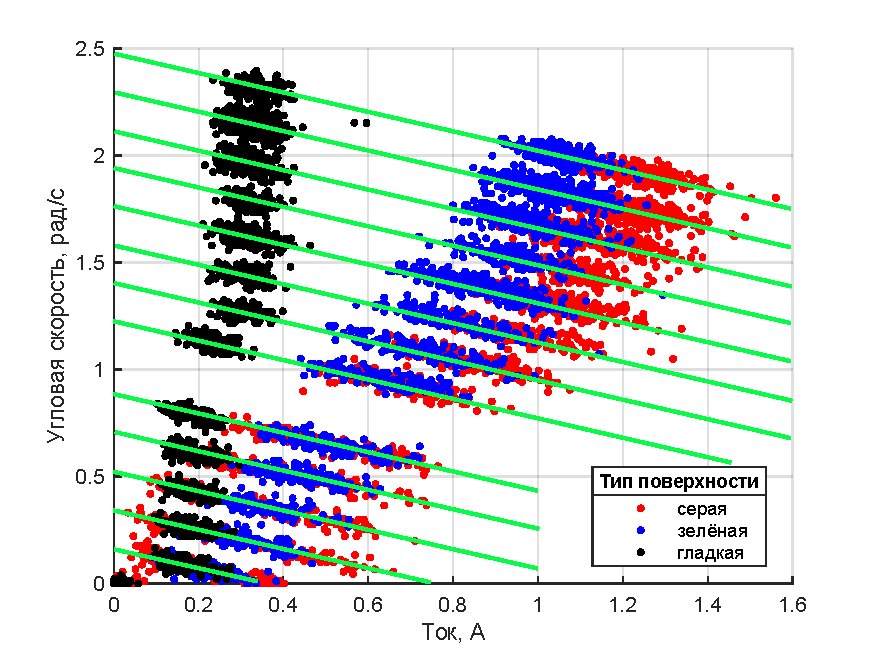
\includegraphics[width=0.6\textwidth]{motor1 electromechanic characteristics.pdf}
    \caption{Примерный вид семейства электромеханических характеристик для 1-го двигателя}
    \label{fig:electromechanic_characteristics}
\end{figure}

\subsection{Зависимость тока от направления движения робота}

\begin{figure}[H]
    \centering
    \begin{subfigure}{0.45\textwidth}
        \centering
        \includegraphics[width=\textwidth]{for_research_movement_direction/polar_current/half_second_averaging/table/motor1.pdf}
        \caption{двигатель 1}
    \end{subfigure}
    \hspace{0.005\textwidth}
    \begin{subfigure}{0.45\textwidth}
        \centering
        \includegraphics[width=\textwidth]{for_research_movement_direction/polar_current/half_second_averaging/table/motor3.pdf}
        \caption{двигатель 3}
    \end{subfigure} \\
    \vspace{4pt}
    \centering
    \begin{subfigure}{0.45\textwidth}
        \centering
        \includegraphics[width=\textwidth]{for_research_movement_direction/polar_current/half_second_averaging/table/motor2.pdf}
        \caption{двигатель 2}
    \end{subfigure}
    \caption{Зависимость тока двигателя от направления движения робота на гладкой поверхности}
\end{figure}

\begin{figure}[H]
    \centering
    \begin{subfigure}{0.49\textwidth}
        \centering
        \includegraphics[width=\textwidth]{for_research_movement_direction/polar_current/half_second_averaging/gray/motor1.pdf}
        \caption{двигатель 1}
    \end{subfigure}
    \hspace{0.005\textwidth}
    \begin{subfigure}{0.49\textwidth}
        \centering
        \includegraphics[width=\textwidth]{for_research_movement_direction/polar_current/half_second_averaging/gray/motor3.pdf}
        \caption{двигатель 3}
    \end{subfigure} \\
    \vspace{4pt}
    \centering
    \begin{subfigure}{0.49\textwidth}
        \centering
        \includegraphics[width=\textwidth]{for_research_movement_direction/polar_current/half_second_averaging/gray/motor2.pdf}
        \caption{двигатель 2}
    \end{subfigure}
    \caption{Зависимость тока двигателя от направления движения робота на серой поверхности}
\end{figure}

\begin{figure}[H]
    \centering
    \begin{subfigure}{0.49\textwidth}
        \centering
        \includegraphics[width=\textwidth]{for_research_movement_direction/polar_current/half_second_averaging/green/motor1.pdf}
        \caption{двигатель 1}
    \end{subfigure}
    \hspace{0.005\textwidth}
    \begin{subfigure}{0.49\textwidth}
        \centering
        \includegraphics[width=\textwidth]{for_research_movement_direction/polar_current/half_second_averaging/green/motor3.pdf}
        \caption{двигатель 3}
    \end{subfigure} \\
    \vspace{4pt}
    \centering
    \begin{subfigure}{0.49\textwidth}
        \centering
        \includegraphics[width=\textwidth]{for_research_movement_direction/polar_current/half_second_averaging/green/motor2.pdf}
        \caption{двигатель 2}
    \end{subfigure}
    \caption{Зависимость тока двигателя от направления движения робота на зелёной поверхности}
\end{figure}

\begin{figure}[H]
    \centering
    \begin{subfigure}{0.49\textwidth}
        \centering
        \includegraphics[width=\textwidth]{for_research_movement_direction/polar_current/half_second_averaging/motor1.pdf}
        \caption{двигатель 1}
    \end{subfigure}
    \hspace{0.005\textwidth}
    \begin{subfigure}{0.49\textwidth}
        \centering
        \includegraphics[width=\textwidth]{for_research_movement_direction/polar_current/half_second_averaging/motor3.pdf}
        \caption{двигатель 3}
    \end{subfigure} \\
    \vspace{4pt}
    \centering
    \begin{subfigure}{0.49\textwidth}
        \centering
        \includegraphics[width=\textwidth]{for_research_movement_direction/polar_current/half_second_averaging/motor2.pdf}
        \caption{двигатель 2}
    \end{subfigure}
    \caption{Сравнение зависимостей тока двигателя от направления движения робота на разных типах поверхности}
\end{figure}

\subsubsection{Зависимость уголовой скорости колеса от направления движения робота}

\begin{figure}[H]
    \centering
    \begin{subfigure}{0.45\textwidth}
        \centering
        \includegraphics[width=\textwidth]{for_research_movement_direction/polar_velocity/half_second_averaging/table/wheel1.pdf}
        \caption{колесо 1}
    \end{subfigure}
    \hspace{0.005\textwidth}
    \begin{subfigure}{0.45\textwidth}
        \centering
        \includegraphics[width=\textwidth]{for_research_movement_direction/polar_velocity/half_second_averaging/table/wheel3.pdf}
        \caption{колесо 3}
    \end{subfigure} \\
    \vspace{4pt}
    \centering
    \begin{subfigure}{0.45\textwidth}
        \centering
        \includegraphics[width=\textwidth]{for_research_movement_direction/polar_velocity/half_second_averaging/table/wheel2.pdf}
        \caption{колесо 2}
    \end{subfigure}
    \caption{Зависимость уголовой скорости колеса от направления движения робота на гладкой поверхности}
\end{figure}

\begin{figure}[H]
    \centering
    \begin{subfigure}{0.49\textwidth}
        \centering
        \includegraphics[width=\textwidth]{for_research_movement_direction/polar_velocity/half_second_averaging/gray/wheel1.pdf}
        \caption{колесо 1}
    \end{subfigure}
    \hspace{0.005\textwidth}
    \begin{subfigure}{0.49\textwidth}
        \centering
        \includegraphics[width=\textwidth]{for_research_movement_direction/polar_velocity/half_second_averaging/gray/wheel3.pdf}
        \caption{колесо 3}
    \end{subfigure} \\
    \vspace{4pt}
    \centering
    \begin{subfigure}{0.49\textwidth}
        \centering
        \includegraphics[width=\textwidth]{for_research_movement_direction/polar_velocity/half_second_averaging/gray/wheel2.pdf}
        \caption{колесо 2}
    \end{subfigure}
    \caption{Зависимость уголовой скорости колеса от направления движения робота на серой поверхности}
\end{figure}

\begin{figure}[H]
    \centering
    \begin{subfigure}{0.49\textwidth}
        \centering
        \includegraphics[width=\textwidth]{for_research_movement_direction/polar_velocity/half_second_averaging/green/wheel1.pdf}
        \caption{колесо 1}
    \end{subfigure}
    \hspace{0.005\textwidth}
    \begin{subfigure}{0.49\textwidth}
        \centering
        \includegraphics[width=\textwidth]{for_research_movement_direction/polar_velocity/half_second_averaging/green/wheel3.pdf}
        \caption{колесо 3}
    \end{subfigure} \\
    \vspace{4pt}
    \centering
    \begin{subfigure}{0.49\textwidth}
        \centering
        \includegraphics[width=\textwidth]{for_research_movement_direction/polar_velocity/half_second_averaging/green/wheel2.pdf}
        \caption{колесо 2}
    \end{subfigure}
    \caption{Зависимость уголовой скорости колеса от направления движения робота на зелёной поверхности}
\end{figure}

Из графиков видно, что ток и угловая скорость имеет похожую зависимость от направления движения робота. При этом, зависимость угловой скорость напрямую обусловлено кинематикой мобильной платформы. А ток в свою очередь зависит уже от задающей скорости/напряжения или выходной скорости. Проверим это.

\subsubsection{Корреляция между угловой скоростью и током двигателя}

\begin{figure}[H]
    \centering
    \begin{subfigure}{0.49\textwidth}
        \centering
        \includegraphics[width=\textwidth]{for_research_movement_direction/correlation_between_motor_current_and_wheel_velocity/table/motor1.pdf}
        \caption{двигатель 1}
    \end{subfigure}
    \hspace{0.005\textwidth}
    \begin{subfigure}{0.49\textwidth}
        \centering
        \includegraphics[width=\textwidth]{for_research_movement_direction/correlation_between_motor_current_and_wheel_velocity/table/motor3.pdf}
        \caption{двигатель 3}
    \end{subfigure} \\
    \vspace{4pt}
    \centering
    \begin{subfigure}{0.49\textwidth}
        \centering
        \includegraphics[width=\textwidth]{for_research_movement_direction/correlation_between_motor_current_and_wheel_velocity/table/motor2.pdf}
        \caption{двигатель 2}
    \end{subfigure}
    \caption{Матрица корреляции между уголовой скоростью и током двигателя на гладкой поверхности}
\end{figure}

\begin{figure}[H]
    \centering
    \begin{subfigure}{0.49\textwidth}
        \centering
        \includegraphics[width=\textwidth]{for_research_movement_direction/correlation_between_motor_current_and_wheel_velocity/gray/motor1.pdf}
        \caption{двигатель 1}
    \end{subfigure}
    \hspace{0.005\textwidth}
    \begin{subfigure}{0.49\textwidth}
        \centering
        \includegraphics[width=\textwidth]{for_research_movement_direction/correlation_between_motor_current_and_wheel_velocity/gray/motor3.pdf}
        \caption{двигатель 3}
    \end{subfigure} \\
    \vspace{4pt}
    \centering
    \begin{subfigure}{0.49\textwidth}
        \centering
        \includegraphics[width=\textwidth]{for_research_movement_direction/correlation_between_motor_current_and_wheel_velocity/gray/motor2.pdf}
        \caption{двигатель 2}
    \end{subfigure}
    \caption{Матрица корреляции между уголовой скоростью и током двигателя на серой поверхности}
\end{figure}

\begin{figure}[H]
    \centering
    \begin{subfigure}{0.49\textwidth}
        \centering
        \includegraphics[width=\textwidth]{for_research_movement_direction/correlation_between_motor_current_and_wheel_velocity/green/motor1.pdf}
        \caption{двигатель 1}
    \end{subfigure}
    \hspace{0.005\textwidth}
    \begin{subfigure}{0.49\textwidth}
        \centering
        \includegraphics[width=\textwidth]{for_research_movement_direction/correlation_between_motor_current_and_wheel_velocity/green/motor3.pdf}
        \caption{двигатель 3}
    \end{subfigure} \\
    \vspace{4pt}
    \centering
    \begin{subfigure}{0.49\textwidth}
        \centering
        \includegraphics[width=\textwidth]{for_research_movement_direction/correlation_between_motor_current_and_wheel_velocity/green/motor2.pdf}
        \caption{двигатель 2}
    \end{subfigure}
    \caption{Матрица корреляции между уголовой скоростью и током двигателя на зелёной поверхности}
\end{figure}

\subsection{Сравнение формы полярных кривых среднего значения тока на каждом направлении}

\begin{figure}[H]
    \centering
    \begin{subfigure}{0.49\textwidth}
        \centering
        \includegraphics[width=\textwidth]{for_research_movement_direction/polar_current/full_averaging/motor1.pdf}
        \caption{двигатель 1}
    \end{subfigure}
    \hspace{0.005\textwidth}
    \begin{subfigure}{0.49\textwidth}
        \centering
        \includegraphics[width=\textwidth]{for_research_movement_direction/polar_current/full_averaging/motor3.pdf}
        \caption{двигатель 3}
    \end{subfigure} \\
    \vspace{4pt}
    \centering
    \begin{subfigure}{0.49\textwidth}
        \centering
        \includegraphics[width=\textwidth]{for_research_movement_direction/polar_current/full_averaging/motor2.pdf}
        \caption{двигатель 2}
    \end{subfigure}
    \caption{Зависимость среднего значения тока от направления движения робота}
\end{figure}

\subsection{Зависимость проскальзывания от направления движения}

\begin{figure}[H]
    \centering
    \begin{subfigure}{0.49\textwidth}
        \centering
        \includegraphics[width=\textwidth]{for_research_movement_direction/polar_slippage/half_second_averaging/table/motor1.pdf}
        \caption{двигатель 1}
    \end{subfigure}
    \hspace{0.005\textwidth}
    \begin{subfigure}{0.49\textwidth}
        \centering
        \includegraphics[width=\textwidth]{for_research_movement_direction/polar_slippage/half_second_averaging/table/motor3.pdf}
        \caption{двигатель 3}
    \end{subfigure} \\
    \vspace{4pt}
    \centering
    \begin{subfigure}{0.49\textwidth}
        \centering
        \includegraphics[width=\textwidth]{for_research_movement_direction/polar_slippage/half_second_averaging/table/motor2.pdf}
        \caption{двигатель 2}
    \end{subfigure}
    \caption{Зависимость проскальзывания от направления движения робота на гладкой поверхности}
\end{figure}

\begin{figure}[H]
    \centering
    \begin{subfigure}{0.49\textwidth}
        \centering
        \includegraphics[width=\textwidth]{for_research_movement_direction/polar_slippage/half_second_averaging/gray/motor1.pdf}
        \caption{двигатель 1}
    \end{subfigure}
    \hspace{0.005\textwidth}
    \begin{subfigure}{0.49\textwidth}
        \centering
        \includegraphics[width=\textwidth]{for_research_movement_direction/polar_slippage/half_second_averaging/gray/motor3.pdf}
        \caption{двигатель 3}
    \end{subfigure} \\
    \vspace{4pt}
    \centering
    \begin{subfigure}{0.49\textwidth}
        \centering
        \includegraphics[width=\textwidth]{for_research_movement_direction/polar_slippage/half_second_averaging/gray/motor2.pdf}
        \caption{двигатель 2}
    \end{subfigure}
    \caption{Зависимость проскальзывания от направления движения робота на серой поверхности}
\end{figure}

\begin{figure}[H]
    \centering
    \begin{subfigure}{0.49\textwidth}
        \centering
        \includegraphics[width=\textwidth]{for_research_movement_direction/polar_slippage/half_second_averaging/green/motor1.pdf}
        \caption{двигатель 1}
    \end{subfigure}
    \hspace{0.005\textwidth}
    \begin{subfigure}{0.49\textwidth}
        \centering
        \includegraphics[width=\textwidth]{for_research_movement_direction/polar_slippage/half_second_averaging/green/motor3.pdf}
        \caption{двигатель 3}
    \end{subfigure} \\
    \vspace{4pt}
    \centering
    \begin{subfigure}{0.49\textwidth}
        \centering
        \includegraphics[width=\textwidth]{for_research_movement_direction/polar_slippage/half_second_averaging/green/motor2.pdf}
        \caption{двигатель 2}
    \end{subfigure}
    \caption{Зависимость проскальзывания от направления движения робота на зелёной поверхности}
\end{figure}

\subsection{Зависимость разницы между скоростью движения робота по энкодерам и камере от направления движения}

\begin{figure}[H]
    \centering
    \begin{subfigure}{0.49\textwidth}
        \centering
        \includegraphics[width=\textwidth]{for_research_movement_direction/polar_delta_speed/half_second_averaging/table/x_axis.pdf}
        \caption{вдоль оси X}
    \end{subfigure}
    \hspace{0.005\textwidth}
    \begin{subfigure}{0.49\textwidth}
        \centering
        \includegraphics[width=\textwidth]{for_research_movement_direction/polar_delta_speed/half_second_averaging/table/y_axis.pdf}
        \caption{вдоль оси Y}
    \end{subfigure} \\
    \vspace{4pt}
    \centering
    \begin{subfigure}{0.49\textwidth}
        \centering
        \includegraphics[width=\textwidth]{for_research_movement_direction/polar_delta_speed/half_second_averaging/table/rotation.pdf}
        \caption{вращательное движение}
    \end{subfigure}
    \caption{Зависимость разницы между скоростью движения робота по энкодерам и камере от направления движения на гладкой поверхности}
\end{figure}

\begin{figure}[H]
    \centering
    \begin{subfigure}{0.49\textwidth}
        \centering
        \includegraphics[width=\textwidth]{for_research_movement_direction/polar_delta_speed/half_second_averaging/gray/x_axis.pdf}
        \caption{вдоль оси X}
    \end{subfigure}
    \hspace{0.005\textwidth}
    \begin{subfigure}{0.49\textwidth}
        \centering
        \includegraphics[width=\textwidth]{for_research_movement_direction/polar_delta_speed/half_second_averaging/gray/y_axis.pdf}
        \caption{вдоль оси Y}
    \end{subfigure} \\
    \vspace{4pt}
    \centering
    \begin{subfigure}{0.49\textwidth}
        \centering
        \includegraphics[width=\textwidth]{for_research_movement_direction/polar_delta_speed/half_second_averaging/gray/rotation.pdf}
        \caption{вращательное движение}
    \end{subfigure}
    \caption{Зависимость разницы между скоростью движения робота по энкодерам и камере от направления движения на серой поверхности}
\end{figure}

\begin{figure}[H]
    \centering
    \begin{subfigure}{0.49\textwidth}
        \centering
        \includegraphics[width=\textwidth]{for_research_movement_direction/polar_delta_speed/half_second_averaging/green/x_axis.pdf}
        \caption{вдоль оси X}
    \end{subfigure}
    \hspace{0.005\textwidth}
    \begin{subfigure}{0.49\textwidth}
        \centering
        \includegraphics[width=\textwidth]{for_research_movement_direction/polar_delta_speed/half_second_averaging/green/y_axis.pdf}
        \caption{вдоль оси Y}
    \end{subfigure} \\
    \vspace{4pt}
    \centering
    \begin{subfigure}{0.49\textwidth}
        \centering
        \includegraphics[width=\textwidth]{for_research_movement_direction/polar_delta_speed/half_second_averaging/green/rotation.pdf}
        \caption{вращательное движение}
    \end{subfigure}
    \caption{Зависимость разницы между скоростью движения робота по энкодерам и камере от направления движения на зелёной поверхности}
\end{figure}

\subsection{Зависимость разницы скоростей по энкодерам и камере от тока по направлению движения}

\begin{figure}[H]
    \centering
    \includegraphics[width=\textwidth]{for_research_movement_direction/robot_delta_speed_vs_axis_current/unsigned_delta_speed/separate_graphs/table/x_axis.pdf}
    \caption{Зависимость разницы скоростей по энкодерам и камере от тока по оси X на гладкой поверхности}
\end{figure}

\begin{figure}[H]
    \centering
    \includegraphics[width=\textwidth]{for_research_movement_direction/robot_delta_speed_vs_axis_current/unsigned_delta_speed/separate_graphs/table/y_axis.pdf}
    \caption{Зависимость разницы скоростей по энкодерам и камере от тока по оси Y на гладкой поверхности}
\end{figure}

\begin{figure}[H]
    \centering
    \includegraphics[width=\textwidth]{for_research_movement_direction/robot_delta_speed_vs_axis_current/unsigned_delta_speed/separate_graphs/table/rotation.pdf}
    \caption{Зависимость разницы скоростей по энкодерам и камере от тока вращательного движения на гладкой поверхности}
\end{figure}

\begin{figure}[H]
    \centering
    \includegraphics[width=\textwidth]{for_research_movement_direction/robot_delta_speed_vs_axis_current/unsigned_delta_speed/separate_graphs/gray/x_axis.pdf}
    \caption{Зависимость разницы скоростей по энкодерам и камере от тока по оси X на серой поверхности}
\end{figure}

\begin{figure}[H]
    \centering
    \includegraphics[width=\textwidth]{for_research_movement_direction/robot_delta_speed_vs_axis_current/unsigned_delta_speed/separate_graphs/gray/y_axis.pdf}
    \caption{Зависимость разницы скоростей по энкодерам и камере от тока по оси Y на серой поверхности}
\end{figure}

\begin{figure}[H]
    \centering
    \includegraphics[width=\textwidth]{for_research_movement_direction/robot_delta_speed_vs_axis_current/unsigned_delta_speed/separate_graphs/gray/rotation.pdf}
    \caption{Зависимость разницы скоростей по энкодерам и камере от тока вращательного движения на серой поверхности}
\end{figure}

\begin{figure}[H]
    \centering
    \includegraphics[width=\textwidth]{for_research_movement_direction/robot_delta_speed_vs_axis_current/unsigned_delta_speed/separate_graphs/green/x_axis.pdf}
    \caption{Зависимость разницы скоростей по энкодерам и камере от тока по оси X на зелёной поверхности}
\end{figure}

\begin{figure}[H]
    \centering
    \includegraphics[width=\textwidth]{for_research_movement_direction/robot_delta_speed_vs_axis_current/unsigned_delta_speed/separate_graphs/green/y_axis.pdf}
    \caption{Зависимость разницы скоростей по энкодерам и камере от тока по оси Y на зелёной поверхности}
\end{figure}

\begin{figure}[H]
    \centering
    \includegraphics[width=0.85\textwidth]{for_research_movement_direction/robot_delta_speed_vs_axis_current/unsigned_delta_speed/separate_graphs/green/rotation.pdf}
    \caption{Зависимость разницы скоростей по энкодерам и камере от тока вращательного движения на зелёной поверхности}
\end{figure}

\begin{figure}[H]
    \centering
    \begin{subfigure}{0.49\textwidth}
        \centering
        \includegraphics[width=\textwidth]{for_research_movement_direction/robot_delta_speed_vs_axis_current/unsigned_delta_speed/common_graphs/x_axis.pdf}
        \caption{вдоль оси X}
    \end{subfigure}
    \hspace{0.005\textwidth}
    \begin{subfigure}{0.49\textwidth}
        \centering
        \includegraphics[width=\textwidth]{for_research_movement_direction/robot_delta_speed_vs_axis_current/unsigned_delta_speed/common_graphs/y_axis.pdf}
        \caption{вдоль оси Y}
    \end{subfigure} \\
    \vspace{4pt}
    \centering
    \begin{subfigure}{0.49\textwidth}
        \centering
        \includegraphics[width=\textwidth]{for_research_movement_direction/robot_delta_speed_vs_axis_current/unsigned_delta_speed/common_graphs/rotation.pdf}
        \caption{вращательное движение}
    \end{subfigure}
    \caption{Сравнение по видам поверхности}
\end{figure}

Если найти результирующий вектор скорости и тока, то получим график, приведённый на рисунке \ref{fig:delta_robot_speed_vector_vs_current_vector}.

\begin{figure}[H]
    \centering
    \includegraphics[width=0.5\textwidth]{for_research_movement_direction/robot_delta_speed_vector_vs_current_vector/common_graphs/all_surface.pdf}
    \caption{Зависимость разницы скоростей по энкодерам и камере от тока для всех поверхностей}
    \label{fig:delta_robot_speed_vector_vs_current_vector}
\end{figure}

\subsection{Зависимость проскальзывания от тока}

\begin{figure}[H]
    \centering
    \begin{subfigure}{0.49\textwidth}
        \centering
        \includegraphics[width=\textwidth]{for_research_movement_direction/wheel_slippage_vs_motor_current/common_graphs/not_linearization/motor1.pdf}
        \caption{двигатель 1}
    \end{subfigure}
    \hspace{0.005\textwidth}
    \begin{subfigure}{0.49\textwidth}
        \centering
        \includegraphics[width=\textwidth]{for_research_movement_direction/wheel_slippage_vs_motor_current/common_graphs/not_linearization/motor2.pdf}
        \caption{двигатель 2}
    \end{subfigure} \\
    \vspace{4pt}
    \centering
    \begin{subfigure}{0.49\textwidth}
        \centering
        \includegraphics[width=\textwidth]{for_research_movement_direction/wheel_slippage_vs_motor_current/common_graphs/not_linearization/motor3.pdf}
        \caption{двигатель 3}
    \end{subfigure}
    \caption{Зависимость проскальзывания от тока двигателя}
\end{figure}

\subsection{Зависимость проскальзывания от тока с учётом вклада колеса в движение робота}

\begin{figure}[H]
    \centering
    \begin{subfigure}{0.50\textwidth}
        \includegraphics[width=\textwidth]{for_research_movement_direction/wheel_slippage_vs_motor_current/common_graphs/not_linearization/motor1.pdf}
        \caption{исходная}
    \end{subfigure} \\
    \begin{subfigure}{0.50\textwidth}
        \includegraphics[width=\textwidth]{for_research_movement_direction/wheel_slippage_vs_motor_current/common_graphs/linearization/motor1.pdf}
        \caption{линеаризованная}
    \end{subfigure}
    \caption{Зависимость проскальзывания от тока 1-го двигателя}
\end{figure}

\begin{figure}[H]
    \centering
    \begin{subfigure}{0.49\textwidth}
        \centering
        \includegraphics[width=\textwidth]{for_research_movement_direction/wheel_slippage_vs_motor_current/common_graphs/linearization/motor1.pdf}
        \caption{двигатель 1}
    \end{subfigure}
    \hspace{0.005\textwidth}
    \begin{subfigure}{0.49\textwidth}
        \centering
        \includegraphics[width=\textwidth]{for_research_movement_direction/wheel_slippage_vs_motor_current/common_graphs/linearization/motor2.pdf}
        \caption{двигатель 2}
    \end{subfigure} \\
    \vspace{4pt}
    \centering
    \begin{subfigure}{0.49\textwidth}
        \centering
        \includegraphics[width=\textwidth]{for_research_movement_direction/wheel_slippage_vs_motor_current/common_graphs/linearization/motor3.pdf}
        \caption{двигатель 3}
    \end{subfigure}
    \caption{Зависимость проскальзывания от тока с учётом вклада колеса в движение робота}
\end{figure}
\section{Зависимость рассогласования направления векторов заданной скорости, скорости по камере и тока}

\subsection{Зависимость рассогласования направления векторов заданной скорости и скорости по камере}

\begin{figure}[H]
    \centering
    \begin{subfigure}{0.49\textwidth}
        \centering
        \includegraphics[width=\textwidth]{for_research_movement_direction/delta_movement_direction/between_set_point_and_camera/table.pdf}
        \caption{гладкая поверхность}
    \end{subfigure}
    \hspace{0.005\textwidth}
    \begin{subfigure}{0.49\textwidth}
        \centering
        \includegraphics[width=\textwidth]{for_research_movement_direction/delta_movement_direction/between_set_point_and_camera/gray.pdf}
        \caption{серая поверхность}
    \end{subfigure} \\
    \vspace{4pt}
    \centering
    \begin{subfigure}{0.49\textwidth}
        \centering
        \includegraphics[width=\textwidth]{for_research_movement_direction/delta_movement_direction/between_set_point_and_camera/green.pdf}
        \caption{зелёная поверхность}
    \end{subfigure}
    \caption{Зависимость рассогласования направления векторов заданной скорости и скорости по камере}
\end{figure}

\begin{figure}[H]
    \centering
    \includegraphics[width=0.8\textwidth]{for_research_movement_direction/delta_movement_direction/between_set_point_and_camera/common_graph.pdf}
    \caption{Зависимость рассогласования направления векторов заданной скорости и скорости по камере}
\end{figure}

\subsection{Зависимость рассогласования направления векторов заданной скорости и тока}

\begin{figure}[H]
    \centering
    \begin{subfigure}{0.49\textwidth}
        \centering
        \includegraphics[width=\textwidth]{for_research_movement_direction/delta_movement_direction/between_set_point_and_current/table.pdf}
        \caption{гладкая поверхность}
    \end{subfigure}
    \hspace{0.005\textwidth}
    \begin{subfigure}{0.49\textwidth}
        \centering
        \includegraphics[width=\textwidth]{for_research_movement_direction/delta_movement_direction/between_set_point_and_current/gray.pdf}
        \caption{серая поверхность}
    \end{subfigure} \\
    \vspace{4pt}
    \centering
    \begin{subfigure}{0.49\textwidth}
        \centering
        \includegraphics[width=\textwidth]{for_research_movement_direction/delta_movement_direction/between_set_point_and_current/green.pdf}
        \caption{зелёная поверхность}
    \end{subfigure}
    \caption{Зависимость рассогласования направления векторов заданной скорости и тока}
\end{figure}

\subsection{Зависимость рассогласования направления векторов скорости по камере и тока}

\begin{figure}[H]
    \centering
    \begin{subfigure}{0.49\textwidth}
        \centering
        \includegraphics[width=\textwidth]{for_research_movement_direction/delta_movement_direction/between_camera_and_current/table.pdf}
        \caption{гладкая поверхность}
    \end{subfigure}
    \hspace{0.005\textwidth}
    \begin{subfigure}{0.49\textwidth}
        \centering
        \includegraphics[width=\textwidth]{for_research_movement_direction/delta_movement_direction/between_camera_and_current/gray.pdf}
        \caption{серая поверхность}
    \end{subfigure} \\
    \vspace{4pt}
    \centering
    \begin{subfigure}{0.49\textwidth}
        \centering
        \includegraphics[width=\textwidth]{for_research_movement_direction/delta_movement_direction/between_camera_and_current/green.pdf}
        \caption{зелёная поверхность}
    \end{subfigure}
    \caption{Зависимость рассогласования направления векторов скорости по камере и тока}
\end{figure}

\begin{figure}[H]
    \centering
    \includegraphics[width=0.8\textwidth]{for_research_movement_direction/delta_movement_direction/between_camera_and_current/common_graph.pdf}
    \caption{Зависимость рассогласования направления векторов скорости по камере и тока}
\end{figure}
\section{Исследование влияния скорости на полученные зависимости}

\subsection{Зависимость разницы скоростей робота по энкодерам и камере от тока по направлению движения}

\begin{figure}[H]
    \centering
    \begin{subfigure}{0.49\textwidth}
        \centering
        \includegraphics[width=\textwidth]{for_research_movement_direction/robot_delta_speed_vs_axis_current/speed_amplitude_influence/x_axis.pdf}
        \caption{по оси X}
    \end{subfigure}
    \hspace{0.005\textwidth}
    \begin{subfigure}{0.49\textwidth}
        \centering
        \includegraphics[width=\textwidth]{for_research_movement_direction/robot_delta_speed_vs_axis_current/speed_amplitude_influence/y_axis.pdf}
        \caption{по оси Y}
    \end{subfigure} \\
    \vspace{4pt}
    \centering
    \begin{subfigure}{0.49\textwidth}
        \centering
        \includegraphics[width=\textwidth]{for_research_movement_direction/robot_delta_speed_vs_axis_current/speed_amplitude_influence/rotation.pdf}
        \caption{для вращательного движения}
    \end{subfigure}
    \caption{Зависимость разницы скоростей робота по энкодерам и камере от тока по направлению движения на разных поверхностях на разных скоростях}
\end{figure}

\subsection{Зависимость разницы скоростей колёс по энкодерам и камере от тока по направлению движения}

\begin{figure}[H]
    \centering
    \begin{subfigure}{0.49\textwidth}
        \centering
        \includegraphics[width=\textwidth]{for_research_movement_direction/wheel_delta_velocity_vs_motor_current/speed_amplitude_influence/motor 1.pdf}
        \caption{двигатель 1}
    \end{subfigure}
    \hspace{0.005\textwidth}
    \begin{subfigure}{0.49\textwidth}
        \centering
        \includegraphics[width=\textwidth]{for_research_movement_direction/wheel_delta_velocity_vs_motor_current/speed_amplitude_influence/motor 2.pdf}
        \caption{двигатель 2}
    \end{subfigure} \\
    \vspace{4pt}
    \centering
    \begin{subfigure}{0.49\textwidth}
        \centering
        \includegraphics[width=\textwidth]{for_research_movement_direction/wheel_delta_velocity_vs_motor_current/speed_amplitude_influence/motor 3.pdf}
        \caption{двигатель 3}
    \end{subfigure}
    \caption{Зависимость разницы скоростей колёс по энкодерам и камере от тока по направлению движения на разных поверхностях на разных скоростях}
\end{figure}

\subsection{Влияние учёта кинематического коэффициента на распределение данных}

\begin{figure}[H]
    \centering
    \begin{subfigure}{0.49\textwidth}
        \centering
        \includegraphics[width=\textwidth]{for_research_movement_direction/wheel_slippage_vs_motor_current/speed_amplitude_influence/not_linearization/motor 1.pdf}
        \caption{без коэффициента}
    \end{subfigure}
    \hspace{0.005\textwidth}
    \begin{subfigure}{0.49\textwidth}
        \centering
        \includegraphics[width=\textwidth]{for_research_movement_direction/wheel_slippage_vs_motor_current/speed_amplitude_influence/linearization/motor 1.pdf}
        \caption{с коэффициентом}
    \end{subfigure}
    \caption{ЗВлияние учёта кинематического коэффициента на распределение данных для двигателя 1}
\end{figure}

\subsection{Зависимость проскальзывания от тока с учётом коэффициента}

\begin{figure}[H]
    \centering
    \begin{subfigure}{0.49\textwidth}
        \centering
        \includegraphics[width=\textwidth]{for_research_movement_direction/wheel_slippage_vs_motor_current/speed_amplitude_influence/linearization/motor 1.pdf}
        \caption{двигатель 1}
    \end{subfigure}
    \hspace{0.005\textwidth}
    \begin{subfigure}{0.49\textwidth}
        \centering
        \includegraphics[width=\textwidth]{for_research_movement_direction/wheel_slippage_vs_motor_current/speed_amplitude_influence/linearization/motor 2.pdf}
        \caption{двигатель 2}
    \end{subfigure} \\
    \vspace{4pt}
    \centering
    \begin{subfigure}{0.49\textwidth}
        \centering
        \includegraphics[width=\textwidth]{for_research_movement_direction/wheel_slippage_vs_motor_current/speed_amplitude_influence/linearization/motor 3.pdf}
        \caption{двигатель 3}
    \end{subfigure}
    \caption{Зависимость проскальзывания от тока с учётом коэффициента на разных поверхностях на разных скоростях}
\end{figure}
\section{Исследование влияния распределения массы робота по колёсам}

{\bfseries Гипотеза:} отличие полученных характеристик для второго двигателя от первого и третьего вызвано неравномерным распределением массы робота. 
Конструкции робота предполагает расположение двух аккумуляторных батарей в задней части робота между первым и вторым и вторым и третьим колёсами, что создаёт дисбаланс распределения массы по колёсам.
Получается, что на второе колесо приходится больше массы, чем на первое и третье.

Для того, чтобы сделать распределение массы по колёсам более равномерным, добавим такую же аккумуляторную батарею в переднюю часть робота между первым и третьим колесом.

\begin{figure}[H]
    \centering
    \begin{subfigure}{0.49\textwidth}
        \centering
        \includegraphics[width=\textwidth]{wheel_load_distribution/polar_current/half_second_averaging/gray motor 1.pdf}
        \caption{двигатель 1}
    \end{subfigure}
    \hspace{0.005\textwidth}
    \begin{subfigure}{0.49\textwidth}
        \centering
        \includegraphics[width=\textwidth]{wheel_load_distribution/polar_current/half_second_averaging/gray motor 3.pdf}
        \caption{двигатель 3}
    \end{subfigure} \\
    \vspace{4pt}
    \centering
    \begin{subfigure}{0.49\textwidth}
        \centering
        \includegraphics[width=\textwidth]{wheel_load_distribution/polar_current/half_second_averaging/gray motor 2.pdf}
        \caption{двигатель 2}
    \end{subfigure}
    \caption{Зависимость тока двигателя от направления движения робота на серой поверхности для неравномерного и равномерного распределение массы}
\end{figure}

\begin{figure}[H]
    \centering
    \begin{subfigure}{0.49\textwidth}
        \centering
        \includegraphics[width=\textwidth]{wheel_load_distribution/polar_current/full_averaging/gray motor 1.pdf}
        \caption{двигатель 1}
    \end{subfigure}
    \hspace{0.005\textwidth}
    \begin{subfigure}{0.49\textwidth}
        \centering
        \includegraphics[width=\textwidth]{wheel_load_distribution/polar_current/full_averaging/gray motor 3.pdf}
        \caption{двигатель 3}
    \end{subfigure} \\
    \vspace{4pt}
    \centering
    \begin{subfigure}{0.49\textwidth}
        \centering
        \includegraphics[width=\textwidth]{wheel_load_distribution/polar_current/full_averaging/gray motor 2.pdf}
        \caption{двигатель 2}
    \end{subfigure}
    \caption{Зависимость среднего значения тока от направления движения робота}
\end{figure}

\begin{figure}[H]
    \centering
    \begin{subfigure}{0.49\textwidth}
        \centering
        \includegraphics[width=\textwidth]{wheel_load_distribution/robot_delta_speed_vs_axis_current/gray/x_axis.pdf}
        \caption{вдоль оси X}
    \end{subfigure}
    \hspace{0.005\textwidth}
    \begin{subfigure}{0.49\textwidth}
        \centering
        \includegraphics[width=\textwidth]{wheel_load_distribution/robot_delta_speed_vs_axis_current/gray/y_axis.pdf}
        \caption{вдоль оси Y}
    \end{subfigure} \\
    \vspace{4pt}
    \centering
    \begin{subfigure}{0.49\textwidth}
        \centering
        \includegraphics[width=\textwidth]{wheel_load_distribution/robot_delta_speed_vs_axis_current/gray/rotation.pdf}
        \caption{вращательное движение}
    \end{subfigure}
    \caption{Сравнение по осям локальной системы координат робота}
\end{figure}

\begin{figure}[H]
    \centering
    \begin{subfigure}{0.49\textwidth}
        \centering
        \includegraphics[width=\textwidth]{wheel_load_distribution/wheel_slippage_vs_motor_current/gray motor 1.pdf}
        \caption{двигатель 1}
    \end{subfigure}
    \hspace{0.005\textwidth}
    \begin{subfigure}{0.49\textwidth}
        \centering
        \includegraphics[width=\textwidth]{wheel_load_distribution/wheel_slippage_vs_motor_current/gray motor 3.pdf}
        \caption{двигатель 3}
    \end{subfigure} \\
    \vspace{4pt}
    \centering
    \begin{subfigure}{0.49\textwidth}
        \centering
        \includegraphics[width=\textwidth]{wheel_load_distribution/wheel_slippage_vs_motor_current/gray motor 2.pdf}
        \caption{двигатель 2}
    \end{subfigure}
    \caption{Сравнение по двигателям}
\end{figure}

\subsection{Измерение силы нормальной реакции опоры на колёсах Robotino 2}

Измерения проводились с помощью кухонных весов с диапазоном измерения \qtyrange{2}{5000}{г}.
Точность измерения весов \qty{1}{г}.

Для измерения силы нормальной реакции опоры или силы давления колеса на опору под одно из колёс робота подкладывались весы, под оставшиеся колёса -- опоры примерно равной с весами высотой.
Это необходимо, чтобы избежать перекоса робота и тем самым повысить точность полученных измерений.

Для проверки разброса значений измерителя был \num{5} раз последовательно взвешен балласт (один из аккумуляторов Robotino).
Балласт в данном случае -- это масса, которая устанавливается на робота в целях равномерно загрузить колёса робота.
Получились следующие показания: \qtylist{1387;1387;1387;1387;1386}{г}.

Были произведены два варианта измерений: без балласта и с балластом.
Показания измерений и оценки погрешности приведены в таблицах \ref{tab:nonuniform_load} и \ref{tab:uniform_load}.

\begin{table}[H]
    \centering
    \caption{Распределение массы робота по колёсам без балласта}
    \label{tab:nonuniform_load}
    \sisetup{
        round-mode = places,
        round-precision = 1
    }%
    \begin{tabular}{S[round-mode = none]SSS}
         & \multicolumn{3}{c}{Распределение массы по колёсам, \unit{г}} \\ \cmidrule(lr){2-4}
        {№ измерения} & {1-ое} & {2-ое} & {3-е} \\
        \midrule
        1 & 2812 & > 5200 & 3268 \\
        2 & 2593 & > 5200 & 3210 \\
        3 & 3433 & 4905 & 2904 \\
        4 & 3616 & 4922 & 2981 \\
        5 & 3045 & > 5200 & 3105 \\
        \midrule
        {среднее} & 3099.8 & 5085.4 & 3093.6 \\
        {среднеквадратическое отклонение} & 424.31 & 157.04 & 152.25 \\
        {доверительные границы (P = 0.95)} & 189.758 & 70.229 & 68.088 \\
    \end{tabular}
\end{table}

\begin{table}[H]
    \centering
    \caption{Распределение массы робота по колёсам с балластом}
    \label{tab:uniform_load}
    \sisetup{
        round-mode = places,
        round-precision = 1
    }%
    \begin{tabular}{S[round-mode = none]SSS}
         & \multicolumn{3}{c}{Распределение массы по колёсам, \unit{г}} \\ \cmidrule(lr){2-4}
        {№ измерения} & {1-ое} & {2-ое} & {3-е} \\
        \midrule
        1 & 3861 & 4663 & 4069 \\
        2 & 3353 & 4630 & 4238 \\
        3 & 3981 & > 5200 & 3517 \\
        4 & 3998 & > 5200 & 3762 \\
        5 & 4235 & > 5200 & 3527 \\
        \midrule
        {среднее} & 3885.6 & 4978.6 & 3822.6 \\
        {среднеквадратическое отклонение} & 327.140 & 303.388 & 323.153 \\
        {доверительные границы (P = 0.95)} & 294.804 & 273.401 & 291.212 \\
    \end{tabular}
\end{table}

Получены следующие оценки распределения массы робота/силы давления по колёсам:
\begin{itemize}
    \item без балласта
    \begin{itemize}
        \item первое колесо: \qty{3099.8 \pm 382.4}{г} или \qty{30.409 \pm 3.751}{Н};
        \item второе колесо: \qty{> 5085.4 \pm 141.5}{г} или \qty{> 49.889 \pm 1.388}{Н};
        \item третье колесо: \qty{3093.6 \pm 137.2}{г} или \qty{30.348 \pm 1.345}{Н};
    \end{itemize}
    \item с балластом
    \begin{itemize}
        \item первое колесо: \qty{3885.6 \pm 294.804}{г} или \qty{38.117 \pm 2.892}{Н};
        \item второе колесо: \qty{> 4978.6 \pm 273.401}{г} или \qty{> 48.840 \pm 2.682}{Н};
        \item третье колесо: \qty{3822.6 \pm 291.212}{г} или \qty{37.499 \pm 2.856}{Н};
    \end{itemize}
\end{itemize}

\end{document}